\documentclass[11pt,addpoints]{exam}
\usepackage[dvipsnames]{xcolor} % Required for custom color
\usepackage{color,colortbl}
\usepackage[utf8]{inputenc}
\usepackage{geometry} % Custom margins
\usepackage[spanish]{babel}
\usepackage{adjustbox,dashbox}
\usepackage{array}
\usepackage{tikz,pgfplots,pgfkeys}
\usepackage{forest,mathtools,siunitx}
\usepackage{amsfonts, amssymb, amsxtra, amsmath, amsbsy}
\usepackage{newclude}
\usepackage{ifthen}
\usepackage{float}
\usepackage{fancybox}
\usepackage{graphicx,tabularx}
\usepackage{multicol,multirow}
\usepackage{enumitem} % Customising the numbered lists
\usepackage{xhfill} % Making the pink block not extend beyond the margin
\usepackage{nameref} % reference the names of the sections
\usepackage{caption,capt-of}
\usepackage[normalem]{ulem} % Dashed lines in appendix
\usepackage{ragged2e} % Ragged left
\usepackage{booktabs}
\usepackage[unboxed]{cwpuzzle}
\usepackage[colorlinks = true,linkcolor = blue]{hyperref}
\usepackage{subfiles}
\usepackage{wrapfig}
\input{insbox}
\usepackage{etoolbox}
\usepackage{mwe}
\usepackage{comfortaa}
\usepackage[T1]{fontenc}
\renewcommand*\oldstylenums[1]{{\firaoldstyle #1}}
\usepackage[T1]{fontenc}
\usepackage{pythontex}
\usepackage{polynom}
\usepackage{longdivision}

 % Imports all the required packages. See Functional/%Packages.tex for more detailS
\usetikzlibrary{arrows.meta}
\usetikzlibrary{shapes.geometric}
\decimalpoint
\makeatletter
\def\maxwidth{%
  \ifdim\Gin@nat@width>\linewidth
    \linewidth
  \else
    \Gin@nat@width
  \fi
}
\makeatother
\pgfplotsset{compat=newest}
\usepgfplotslibrary{groupplots}
\usetikzlibrary{
  arrows,
  positioning,
  matrix,
  calc,
  decorations.pathreplacing,
  decorations.pathmorphing,
  decorations.markings,
  decorations.text,
  shapes,
  backgrounds,
  shadows,
  trees,
  fit,
  snakes,
  patterns,
  mindmap,
  intersections,
  calendar,
  plotmarks,
  spy}

\pagestyle{empty}

% Deve vir depois de pagestyle{}.
\definecolor{darkgreen}{rgb}{0.13,0.53,0.53}
\definecolor{fgcolor}{rgb}{0.345, 0.345, 0.345}
% \definecolor{fgcolor}{rgb}{0.5, 0.5, 0.5}
\newcommand{\hlnum}[1]{\textcolor[rgb]{0.686,0.059,0.569}{#1}}%
\newcommand{\hlstr}[1]{\textcolor[rgb]{0.192,0.494,0.8}{#1}}%
\newcommand{\hlcom}[1]{\textcolor[rgb]{0.678,0.584,0.686}{\textit{#1}}}%
\newcommand{\hlopt}[1]{\textcolor[rgb]{0,0,0}{#1}}%
\newcommand{\hlstd}[1]{\textcolor[rgb]{0.345,0.345,0.345}{#1}}%
\newcommand{\hlkwa}[1]{\textcolor[rgb]{0.161,0.373,0.58}{\textbf{#1}}}%
\newcommand{\hlkwb}[1]{\textcolor[rgb]{0.69,0.353,0.396}{#1}}%
\newcommand{\hlkwc}[1]{\textcolor[rgb]{0.333,0.667,0.333}{#1}}%
\newcommand{\hlkwd}[1]{\textcolor[rgb]{0.737,0.353,0.396}{\textbf{#1}}}%
\definecolor{cielo}{HTML}{00ACD1}
\definecolor{colorrds}{HTML}{0060A0} % Custom colour
\definecolor{cadmiumgreen}{rgb}{0.0, 0.42, 0.24}
\definecolor{cadmiumorange}{rgb}{0.93, 0.53, 0.18}
\definecolor{SolutionBoxColor}{gray}{0.8}
\definecolor{purplePoint}{HTML}{7A52E1}
\def\LOGO{%
  \begin{picture}(0,0)\unitlength=1cm
    \put (3,-1.5) {
\includegraphics[width=2.5cm]{./Images/LOGO_RDS.jpg}}
  \end{picture}
}
\def\arraystretch{1.5}
\definecolor{shadecolor}{rgb}{.97, .97, .97}
\definecolor{messagecolor}{rgb}{0, 0, 0}
\definecolor{warningcolor}{rgb}{1, 0, 1}
\definecolor{errorcolor}{rgb}{1, 0, 0}
\newenvironment{knitrout}{}{}
\tikzset{
  abstractbox/.style={
    draw=black, fill=white, rectangle, 
    inner sep=12pt, style=rounded corners,
    drop shadow={fill=black, opacity=1}
  },
  abstracttitle/.style={fill=white}
}
\usepackage{framed}
\makeatletter
\newenvironment{kframe}{%
  \def\at@end@of@kframe{}%
  \ifinner\ifhmode%
  \def\at@end@of@kframe{\end{minipage}}%
\begin{minipage}{\columnwidth}%
  \fi\fi%
  \def\FrameCommand##1{\hskip\@totalleftmargin \hskip-\fboxsep
    % \colorbox{shadecolor}{##1}\hskip-\fboxsep
    ##1 \hskip-\fboxsep
    % There is no \\@totalrightmargin, so:
    \hskip-\linewidth \hskip-\@totalleftmargin \hskip\columnwidth}%
  \MakeFramed {\advance\hsize-\width
    \@totalleftmargin\z@ \linewidth\hsize
    \@setminipage}}%
{\par\unskip\endMakeFramed%
  \at@end@of@kframe}
\makeatother
\newcommand{\boxabstract}[2][fill=white]{
  \begin{tikzpicture}
    \node [abstractbox, #1] (box)
    {\begin{minipage}{0.9\linewidth}
        \setlength{\parindent}{2mm} % Indentar.
        \normalfont #2
      \end{minipage}};
    \node[abstracttitle, right=10pt] at (box.north west) {Instrucciones};
    \node[draw=none, fit=(box)] {};
  \end{tikzpicture}
}
\renewcommand{\solutiontitle}{\textbf{Soluci\'on:}\par\noindent}
\newcommand{\tf}[1][{}]{%
\fillin[#1][1cm]%
}
\newcommand*\circled[1]{\tikz[baseline=(char.base)]{%
    \node[shape=circle, draw, minimum size=1.5em, inner sep=0pt, label={center:#1}, thick] (char) {#1};}}
\renewcommand\choicelabel{%
  \circled{\thechoice}}
\longdivisionkeys{style=standard}

\usepackage{alltt}

% Tamanho de fonte e distância entre linhas.
\renewenvironment{knitrout}{
  \footnotesize\renewcommand{\baselinestretch}{0.75}
}{}

\AtBeginEnvironment{choices}{\vspace{0.1\baselineskip}}
\AtEndEnvironment{choices}{\vspace{0.8\baselineskip}}
\AtBeginEnvironment{oneparchoices}{\vspace{0.1\baselineskip}}
\AtEndEnvironment{oneparchoices}{\vspace{0.8\baselineskip}} 
\AtBeginEnvironment{checkboxes}{\vspace{0.1\baselineskip}}
\AtEndEnvironment{checkboxes}{\vspace{0.8\baselineskip}}
\AtBeginEnvironment{oneparcheckboxes}{\vspace{0.1\baselineskip}}
\AtEndEnvironment{oneparcheckboxes}{\vspace{0.8\baselineskip}} 


\geometry{letterpaper,total={175mm,220mm},left=15mm,top=15mm,} % Custom margins
\pgfplotsset{compat=1.17}
\footer{}{\thepage}{}
%\captionsetup{width=.45\textwidth}
\setlength{\parindent}{0pt}
\graphicspath{{../Images}} %Setting the graphicspath
\checkboxchar{$\Box$}
\bracketedpoints
\pointpoints{punto}{puntos}
\hqword{Pregunta}
\hpgword{P\'gina}
\hpword{Puntos}
%\chbpword{Puntos extra}
\hsword{Puntos obtenidos}
\htword{Total}

\newenvironment{mybox}[3][]{%
  \begin{tikzpicture}[#1]%
    \def\myboxname{#3}%
    % good options: minimum height, minimum width
    \node [draw, inner sep=0ex,  align=justify, draw=none]
      (BOXCONTENT) \bgroup\rule{0ex}{0ex}\ignorespaces
  }{%
    \egroup;
    \node [right, inner sep=3pt, fill=colorrds!75, outer sep=0pt, 
      text height=2ex, text depth=.5ex] (BOXNAME) 
      at ([shift={(-1em,5pt)}]BOXCONTENT.north west) {\myboxname};
    \fill[colorrds] (BOXNAME.north east) -- +(-1em,1em)
      -- +(-1em,0) -- cycle;
    \fill[colorrds] (BOXNAME.south west) -- +(1em,-1em)
      -- +(1em,0) -- cycle;
  \end{tikzpicture}
}

\begin{document}
\include*{Functional/TitlePage_EXM3U1}
\begin{questions}
    \question[10] Analiza la figura \ref{fig:lados_sem03} y encuentra la medida de $x$.

    \begin{minipage}{0.45\linewidth}
        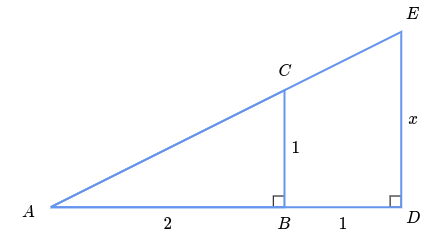
\includegraphics[width=\linewidth]{Images/lados_sem03}
        \captionof{figure}{}
        \label{fig:lados_sem03}
    \end{minipage}\hfill
    \begin{minipage}{0.5\linewidth}
        \begin{solutionbox}{10cm}
            Tanto $\triangle ABC$ como $\triangle ADE$ tiene un ángulo recto y comparten $\angle BAC$.\\

            $\Rightarrow$ $\triangle ABC$ y $\triangle ADE$ son semejantes.\\

            \quad $\therefore$
            \quad $\dfrac{\overline{AB}}{\overline{BC}}=\dfrac{2}{1}=2$ \quad y \quad $\dfrac{\overline{AD}}{\overline{DE}}=\dfrac{2+1}{x}=\dfrac{3}{x}$
            \begin{align*}
                \dfrac{2+x}{11} & =\dfrac{2}{1}  \\
                \dfrac{3}{x}    & =2             \\
                3               & =2x            \\
                x               & = \dfrac{3}{2} \\
            \end{align*}
        \end{solutionbox}
    \end{minipage}%

    \newpage

    \question[20] Observa las siguientes parejas de tri\'angulos y responde a los cuestionamientos.

    %\begin{multicols}{2}
    \begin{parts}
        \part En la figura \ref{fig:triang_sem02}, el triángulo {\color{cielogris}FGH} es semejante al triángulo {\color{strawberry}DEF}. ¿Cuál es el valor de $p$?

        \begin{minipage}[t]{0.5\linewidth}
            \begin{figure}[H]
                \raggedright
                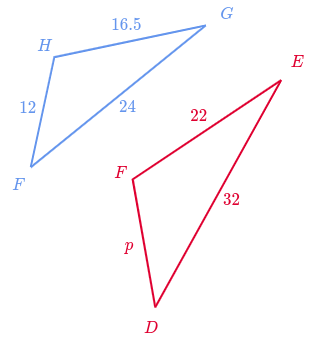
\includegraphics[width =0.9\linewidth ]{Images/triang_sem02}
                \caption{}
                \label{fig:triang_sem02}
            \end{figure}
        \end{minipage}%
        \begin{minipage}[t]{0.5\linewidth}
            \begin{solutionbox}{7cm}
                Los triángulos semejantes tienen lados proporcionales.

                $\Rightarrow$ podemos establecer proporciones equivalentes y resolver para $k$.

                $\therefore$
                \[
                    \dfrac{k}{24} =\dfrac{14}{28} \]    y  \[k =12\]
            \end{solutionbox}
        \end{minipage}

        \part En la figura \ref{fig:triang_sem04}, el triángulo {\color{cielogris}FGH} es semejante al triángulo {\color{strawberry}PQR}. ¿Cuál es el valor de $y$?

        \begin{minipage}[t]{0.5\linewidth}
            \begin{solutionbox}{7cm}

            \end{solutionbox}
        \end{minipage}
        \begin{minipage}[t]{0.5\linewidth}
            \begin{figure}[H]
                \raggedleft
                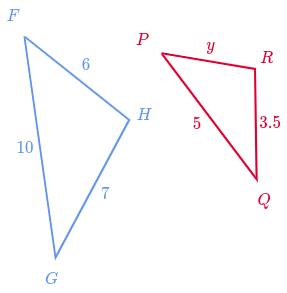
\includegraphics[width =0.9\linewidth ]{Images/triang_sem04}
                \caption{}
                \label{fig:triang_sem04}
            \end{figure}
        \end{minipage}
    \end{parts}
    %\end{multicols}
    \newpage
    \include*{Questions/question009}
    \include*{Questions/question008}
    %\include*{Questions/question010}

    % \question[10] Calcula la longitud de $x$ para cada uno de los siguientes incisos.


    % \begin{multicols}{2}
    %     \begin{parts}
    %         \subfile{Questions/Parts/question013a}
    %         % \subfile{Questions/Parts/question013b}
    %         % \subfile{Questions/Parts/question013c}
    %         % \subfile{Questions/Parts/question013d}
    %     \end{parts}
    % \end{multicols}

    \question[10] Realiza la siguiente multiplicaci\'on de expresiones algebraicas.

    \[(2x^2-4)\cdot(-3x^2-4+10)\]

    %\begin{minipage}[c]{0.5\linewidth}
    \begin{solutionbox}{5.5cm}
        \[ \begin{array}{*{16}{@{}>{{}}r<{{}}@{}}}
                 &  &   & \multirow{2.5}{*}{$ {}\times{} $} &  & - & 3x^2 &  & - & 4x    &  & + & 10  &   &    &    \\
                 &  &   &                                   &  &   &      &  &   & 2x^2  &  & - & 4   &   &    &    \\
                \cmidrule[0.6pt](l{-1pt}r{-1pt}){1-16}
                 &  &   &                                   &  &   &      &  & + & 12x^2 &  & + & 16x &   & -  & 40 \\
                 &  & - & 6x^4                              &  & - & 8x^3 &  & + & 20x^2 &  &   &     &   &    &    \\
                \cmidrule[0.6pt](l{-1pt}r{-1pt}){1-16}
                 &  & - & 6x^4                              &  & - & 8x^3 &  & - & 32x^2 &  & + & 16x & - & 40 &
            \end{array}
        \]
        % \begin{align*}
        %     (2x^2-4)\cdot(-3x^2+4x-10) & = -6x^4+8x^3-20x^2+12x^2-16x+40 \\
        %                                & = -6x^4+8x^3-8x^2-16x+40
        % \end{align*}
    \end{solutionbox}
    %\end{minipage}

    \newpage
    \question[20] En una escuela hay 160 niñas y 120 niños. Se quiere dividir en grupos del mismo tamaño,
    en donde cada grupo tenga el mismo número de niñas y el mismo número de niños. Si la escuela quiere formar el mayor número de grupos posible
    y no quiere que ningún alumno o alumna quede fuera,

    \begin{parts}
        \part ¿Cuántos equipos deberá formar?
        \begin{solutionbox}{6.5cm}
            \begin{minipage}{0.2\textwidth}
                \small
                \begin{tabular}{ cc|c }
                    160 & 120 & \circled{2} \\
                    80  & 60  & \circled{2} \\
                    40  & 30  & \circled{2} \\
                    20  & 15  & \circled{5} \\
                    4   & 3   & 2           \\
                    2   & 3   & 2           \\
                    1   & 3   & 3           \\
                    1   & 1   &             \\
                \end{tabular}
            \end{minipage}%
            \begin{minipage}[b]{0.75\linewidth}
                El mayor número de grupos que se pueden
                constituir de forma entera con 160 y con 120; es decir, el m\'aximo com\'un divisor (MCD) de 160 y 120.

                $\Rightarrow$

                MCD(160,120)$=2^3\times5=40$

                $\therefore$ la cantidad de grupos son: 40

            \end{minipage}
        \end{solutionbox}

        \part ¿Cuántos ni\~nos y niñas habrá en cada equipo?
        \begin{solutionbox}{2cm}
            $\frac{160}{40}=4$  y  $\frac{120}{4}=3$
        \end{solutionbox}

    \end{parts}

\end{questions}
\end{document}
